% Workshop 1 slides. Build with: pdflatex workshop1.tex
%
% Style is base beamer + a custom colour scheme so we don't depend on
% Metropolis or system fonts. Render with a vanilla TeX Live install.

\documentclass[aspectratio=169,11pt]{beamer}
\usefonttheme{professionalfonts}
\usepackage[T1]{fontenc}
\usepackage{lmodern}
\usepackage{tikz}
\usepackage{listings}
\usepackage{xcolor}
\usepackage{booktabs}

\usetikzlibrary{positioning, arrows.meta, calc, fit, backgrounds, shapes.geometric, decorations.pathreplacing}

% --- clean look --------------------------------------------------------
\setbeamertemplate{navigation symbols}{}
\setbeamertemplate{footline}[frame number]
\setbeamertemplate{itemize items}[circle]
\setbeamertemplate{itemize subitem}[triangle]

\definecolor{accent}{HTML}{2C5282}
\definecolor{accent2}{HTML}{B7791F}
\definecolor{muted}{HTML}{4A5568}
\definecolor{codebg}{HTML}{F7FAFC}

\setbeamercolor{frametitle}{fg=accent}
\setbeamercolor{title}{fg=accent}
\setbeamercolor{structure}{fg=accent}
\setbeamercolor{normal text}{fg=black!88}
\setbeamerfont{frametitle}{series=\bfseries, size=\Large}
\setbeamerfont{title}{series=\bfseries, size=\huge}

% --- code listings -----------------------------------------------------
\lstdefinestyle{py}{
  language=Python,
  basicstyle=\ttfamily\footnotesize,
  keywordstyle=\color{accent}\bfseries,
  commentstyle=\color{muted}\itshape,
  stringstyle=\color{accent2},
  showstringspaces=false,
  frame=single,
  framerule=0pt,
  framesep=6pt,
  backgroundcolor=\color{codebg},
  rulecolor=\color{codebg},
  xleftmargin=6pt,
  xrightmargin=6pt,
}
\lstset{style=py}

% reference to a source location, displayed in muted grey
\newcommand{\srcref}[1]{{\color{muted}\ttfamily\footnotesize #1}}

\title{Training a Machine Learning Interatomic Potential}
\date{}
\author{}

\begin{document}

% ----------------------------------------------------------------------
\begin{frame}[plain]
  \titlepage
\end{frame}

% ----------------------------------------------------------------------
\begin{frame}{What we are building}
  \begin{columns}[T]
    \column{0.55\textwidth}
      A function from atoms to
      \begin{itemize}
        \item energy $E$ (eV)
        \item force $\vec{F}_i$ per atom (eV/\AA)
        \item with the right symmetries
      \end{itemize}

      \vspace{0.8em}
      Trained on DFT data; can reach DFT accuracy where hand-coded
      force fields plateau.

    \column{0.45\textwidth}
      \centering
      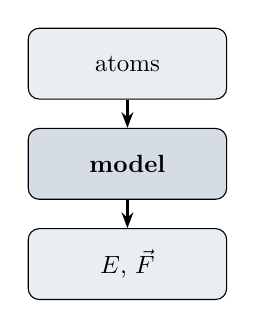
\begin{tikzpicture}[node distance=0.4cm, scale=0.9, transform shape]
        \node[draw, rounded corners, fill=accent!10, minimum width=2.8cm, minimum height=1cm] (input) {atoms};
        \node[below=of input, draw, rounded corners, fill=accent!20, minimum width=2.8cm, minimum height=1cm] (model) {\textbf{model}};
        \node[below=of model, draw, rounded corners, fill=accent!10, minimum width=2.8cm, minimum height=1cm] (output) {$E$, $\vec{F}$};
        \draw[-{Stealth[length=2mm]}, thick] (input) -- (model);
        \draw[-{Stealth[length=2mm]}, thick] (model) -- (output);
      \end{tikzpicture}
  \end{columns}
\end{frame}

% ----------------------------------------------------------------------
\begin{frame}[fragile]{A "frame" is one configuration}
  \vspace{-0.3em}
\begin{lstlisting}
@dataclass
class Frame:
    positions: torch.Tensor       # (N, 3) Angstroms
    atomic_numbers: torch.Tensor  # (N,) long
    energy: torch.Tensor          # scalar, eV
    forces: torch.Tensor          # (N, 3), eV/A
    n_atoms: int
\end{lstlisting}
  \vspace{0.4em}
  \srcref{workshop1/frames.py:33}

  \vspace{0.8em}
  Our training set is 1600 frames of ethanol; validation is 400.
  Every frame has $N=9$ atoms, $E$ in eV, and DFT-computed forces.
\end{frame}

% ----------------------------------------------------------------------
\begin{frame}{The data path, end to end}
  \vspace{-0.5em}
  \centering
  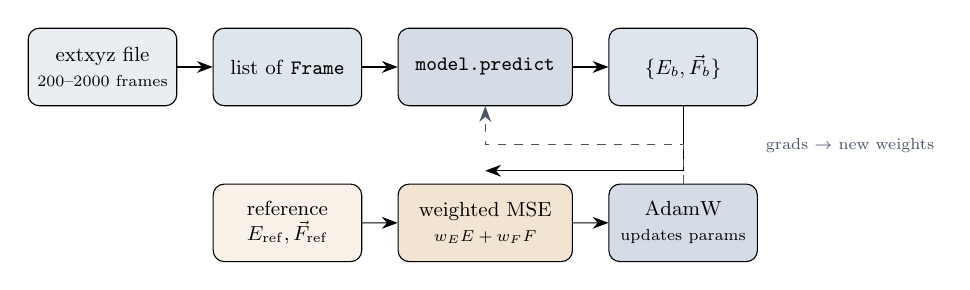
\begin{tikzpicture}[node distance=0.55cm and 0.55cm, scale=0.82, transform shape,
      every node/.style={align=center, font=\small}]

    \node[draw, rounded corners, fill=accent!10, minimum height=1.2cm, minimum width=2.3cm] (xyz) {extxyz file \\ \scriptsize{200--2000 frames}};
    \node[right=of xyz, draw, rounded corners, fill=accent!15, minimum height=1.2cm, minimum width=2.3cm] (frame) {list of \texttt{Frame}};
    \node[right=of frame, draw, rounded corners, fill=accent!20, minimum height=1.2cm, minimum width=2.7cm] (pred) {\texttt{model.predict}};
    \node[right=of pred, draw, rounded corners, fill=accent!15, minimum height=1.2cm, minimum width=2.3cm] (out) {$\{E_b, \vec{F}_b\}$};

    \node[below=1.2cm of pred, draw, rounded corners, fill=accent2!20, minimum height=1.2cm, minimum width=2.7cm] (loss) {weighted MSE \\ \scriptsize{$w_E E + w_F F$}};
    \node[left=of loss, draw, rounded corners, fill=accent2!10, minimum height=1.2cm, minimum width=2.3cm] (ref) {reference \\ $E_{\mathrm{ref}}, \vec{F}_{\mathrm{ref}}$};
    \node[right=of loss, draw, rounded corners, fill=accent!20, minimum height=1.2cm, minimum width=2.3cm] (opt) {AdamW \\ \scriptsize{updates params}};

    \draw[-{Stealth[length=2mm]}] (xyz) -- (frame);
    \draw[-{Stealth[length=2mm]}] (frame) -- (pred);
    \draw[-{Stealth[length=2mm]}] (pred) -- (out);
    \draw[-{Stealth[length=2mm]}] (out) |- ([yshift=2mm]loss.north);
    \draw[-{Stealth[length=2mm]}] (ref) -- (loss);
    \draw[-{Stealth[length=2mm]}] (loss) -- (opt);
    \draw[-{Stealth[length=2mm]}, dashed, color=muted] (opt.north) -- ++(0,0.6) -| (pred.south);
    \node[color=muted, font=\scriptsize, right=0pt of opt, yshift=1.2cm] {grads $\to$ new weights};
  \end{tikzpicture}

  \vspace{0.4em}
  \srcref{workshop1/train.py:166--180  (epoch loop)}
\end{frame}

% ----------------------------------------------------------------------
\begin{frame}[fragile]{The training loop, in one screen}
\begin{lstlisting}
for epoch in range(epochs):
    for start in range(0, n, batch_size):
        batch = train_frames[order[start:start+batch_size]]
        opt.zero_grad()
        loss = w_E * MSE_E(batch) + w_F * MSE_F(batch)
        loss.backward()
        opt.step()
\end{lstlisting}
  \vspace{0.4em}
  \srcref{workshop1/train.py:166--180}

  \vspace{0.8em}
  Outer loop = \textbf{epoch}. Inner loop = \textbf{batch}. \\
  Architecture, loss recipe, optimiser schedule all hang off this.
\end{frame}

% ----------------------------------------------------------------------
\begin{frame}{Epoch vs batch}
  \begin{columns}[T]
    \column{0.5\textwidth}
      \textbf{Epoch} \\
      One full pass through the training set.

      \vspace{0.4em}
      With 1600 train frames and batch size 200, \\
      that's $\lceil 1600 / 200 \rceil = 8$ gradient steps.

      \vspace{0.6em}
      Reasonable target: $\sim$1000 epochs.

    \column{0.5\textwidth}
      \textbf{Batch} \\
      A subset of training data the optimiser sees in one step.

      \vspace{0.4em}
      Larger batch
      \begin{itemize}
        \item less noisy gradient, smoother loss curve
        \item more memory, more GPU work per step
        \item fewer optimiser steps per epoch
      \end{itemize}

      For workshop1, full-batch is fine: 1600 frames \\
      $\times$ 9 atoms is trivial.
  \end{columns}

  \vspace{0.8em}
  \centering
  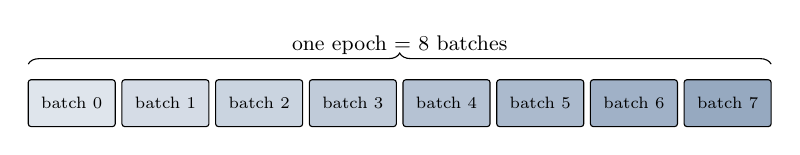
\begin{tikzpicture}[scale=0.85, transform shape]
    \foreach \i in {0,...,7} {
      \draw[fill=accent!\the\numexpr15 + \i*5\relax, rounded corners=1pt]
        (\i*1.4,0) rectangle ++(1.3, 0.7);
      \node[font=\scriptsize] at (\i*1.4 + 0.65, 0.35) {batch \i};
    }
    \draw[decorate, decoration={brace, amplitude=4pt, raise=2pt}]
      (0,0.85) -- (11.1,0.85) node[midway, above=0.3em, font=\small] {one epoch = 8 batches};
  \end{tikzpicture}
\end{frame}

% ----------------------------------------------------------------------
\begin{frame}{Stochastic gradient descent}
  The loss is an average over the $N$ training frames --- so is its
  gradient:
  \[
    L(\theta) = \frac{1}{N}\sum_{i=1}^{N} \ell_i(\theta)
    \qquad
    \nabla L(\theta) = \frac{1}{N}\sum_{i=1}^{N} \nabla \ell_i(\theta)
  \]

  The exact gradient is $N$ per-frame gradients, every step
  ($N=1600$ here; millions for real datasets).

  \vspace{0.6em}
  A \textbf{batch} of $B \ll N$ frames gives an unbiased estimate:
  \[
    \nabla L(\theta) \;\approx\; \frac{1}{B}\sum_{i \in \text{batch}} \nabla \ell_i(\theta)
  \]

  Cheaper per step, noisier direction, more steps --- and the noise
  helps (regularises, escapes sharp minima). Full-batch ($B=N$) is
  exact; fine when $N$ is small, as here.
\end{frame}

% ----------------------------------------------------------------------
\begin{frame}[fragile]{The loss, exactly}
\begin{lstlisting}
def _batch_loss(model, batch, recipe):
    out = model.predict(batch)
    ref_E = stack([fr.energy for fr in batch])
    ref_F = stack([fr.forces for fr in batch])
    L_E = ((out["energies"] - ref_E) / n_atoms).pow(2).mean()
    L_F = (out["forces"]  - ref_F).pow(2).sum() / (3 * n_atoms * B)
    return recipe.w_E * L_E + recipe.w_F * L_F
\end{lstlisting}
  \vspace{0.4em}
  \srcref{workshop1/train.py:105--132}

  \vspace{0.6em}
  Two scalars per batch: $L_E$, $L_F$. We weight them and sum.
  Everything that follows --- AdamW, the schedule, EMA --- is just
  machinery for minimising this expression.
\end{frame}

% ----------------------------------------------------------------------
\begin{frame}{Why divide by $N_{\mathrm{atoms}}$}
  Total energies grow with system size. \\
  A 200-atom box has $\sim$200$\times$ the energy of a single molecule.

  \vspace{0.6em}
  If we squared the raw error, the big box would dominate the loss and
  the small one would barely contribute.

  \vspace{0.6em}
  \textbf{Per-atom normalisation} ($E / N_{\mathrm{atoms}}$) puts every
  system on the same scale: a 9-atom ethanol and a 200-atom water cluster
  contribute equally, regardless of size.

  \vspace{0.8em}
  \srcref{workshop1/train.py:120  ((out["energies"] - ref\_E) / n\_atoms)}
\end{frame}

% ----------------------------------------------------------------------
\begin{frame}{Forces are gradients}
  No special head for forces. We \emph{differentiate} the energy.

  \vspace{0.6em}
  \begin{center}
    \large $\vec{F}_i \;=\; -\dfrac{\partial E}{\partial \vec{r}_i}$
  \end{center}

  \vspace{0.6em}
  \begin{itemize}
    \item \texttt{predict()} sets \texttt{positions.requires\_grad\_(True)}
    \item runs the energy forward pass
    \item calls \texttt{torch.autograd.grad(E, positions)}
    \item returns minus that gradient as the force
  \end{itemize}

  \vspace{0.4em}
  Energy conservation falls out for free.

  \vspace{0.6em}
  \srcref{workshop1/models/pair\_morse.py:153  (autograd.grad call)}
\end{frame}

% ----------------------------------------------------------------------
\begin{frame}{The recipe sweep}
  \texttt{train.py} runs the same model \textbf{five times}, varying only
  the loss weights:

  \vspace{0.6em}
  \centering
  \small
  \begin{tabular}{lccl}
    \toprule
    recipe & $w_E$ & $w_F$ & teaches \\
    \midrule
    E only        & 1   & 0   & energies pin baseline, forces ignored \\
    F only        & 0   & 1   & forces drive shape; $E$ off by a const \\
    E:F = 1:1     & 1   & 1   & balanced --- both fit, both compromise \\
    E:F = 1:100   & 1   & 100 & MACE's canonical default \\
    E:F = 100:1   & 100 & 1   & energies dominate, forces drift \\
    \bottomrule
  \end{tabular}

  \vspace{0.8em}
  \centering
  \textbf{The loss you write down is the model you get.}
\end{frame}

% ----------------------------------------------------------------------
\begin{frame}[fragile]{Four architectures, one interface}
  \vspace{-0.2em}
  \centering
  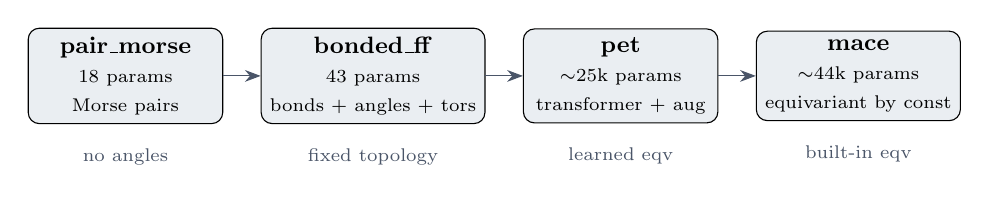
\begin{tikzpicture}[scale=0.95, transform shape,
      every node/.style={font=\small, align=center},
      box/.style={draw, rounded corners, fill=accent!10, minimum width=2.6cm, minimum height=1.15cm}]
    \node[box] (pm) {\textbf{pair\_morse} \\ \scriptsize 18 params \\ \scriptsize Morse pairs};
    \node[box, right=0.5cm of pm] (bf) {\textbf{bonded\_ff} \\ \scriptsize 43 params \\ \scriptsize bonds + angles + tors};
    \node[box, right=0.5cm of bf] (pet) {\textbf{pet} \\ \scriptsize $\sim$25k params \\ \scriptsize transformer + aug};
    \node[box, right=0.5cm of pet] (mace) {\textbf{mace} \\ \scriptsize $\sim$44k params \\ \scriptsize equivariant by const};
    \draw[-{Stealth[length=2mm]}, color=muted] (pm) -- (bf);
    \draw[-{Stealth[length=2mm]}, color=muted] (bf) -- (pet);
    \draw[-{Stealth[length=2mm]}, color=muted] (pet) -- (mace);
    \node[below=0.2cm of pm, font=\scriptsize, color=muted] {no angles};
    \node[below=0.2cm of bf, font=\scriptsize, color=muted] {fixed topology};
    \node[below=0.2cm of pet, font=\scriptsize, color=muted] {learned eqv};
    \node[below=0.2cm of mace, font=\scriptsize, color=muted] {built-in eqv};
  \end{tikzpicture}

  \vspace{0.6em}
  Each implements one method:
  \vspace{-0.4em}
\begin{lstlisting}
def predict(self, frames):
    return {"energies": (B,) tensor,
            "forces":   list of (N_i, 3) tensors}
\end{lstlisting}
  \srcref{workshop1/models/\_\_init\_\_.py:1}
\end{frame}

% ----------------------------------------------------------------------
\begin{frame}{Same loss recipe, different architectures}
  \texttt{compare\_models.py} answers the orthogonal question.

  \vspace{0.6em}
  \centering
  \small
  \begin{tabular}{lrrr}
    \toprule
    model & \#params & RMSE\_E meV/atom & RMSE\_F meV/\AA \\
    \midrule
    pair\_morse  &     18 & high & high \\
    bonded\_ff   &     43 & low  & mid  \\
    pet          & $\sim$25k & low  & mid  \\
    mace         & $\sim$44k & low  & \textbf{best} \\
    \bottomrule
  \end{tabular}

  {\color{muted}\scriptsize (run it for live numbers --- they depend on epochs, precision, hardware)}

  \vspace{0.6em}
  \small
  \begin{itemize}
    \item \textbf{pair\_morse $\to$ bonded\_ff:} angles enter; both metrics jump.
    \item \textbf{bonded\_ff $\to$ pet:} far more params, marginal gain.
    \item \textbf{pet $\to$ mace:} similar budget, built-in equivariance, best forces.
  \end{itemize}
\end{frame}

% ----------------------------------------------------------------------
\begin{frame}{From training to MD}
  Once you have a trained checkpoint:

  \vspace{0.6em}
  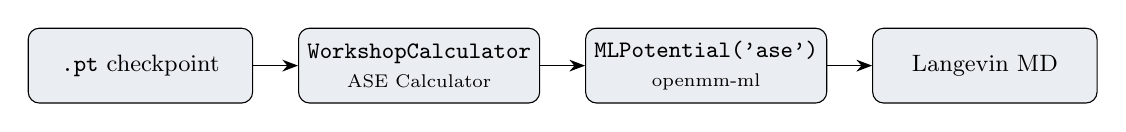
\begin{tikzpicture}[node distance=0.6cm, scale=0.95, transform shape,
      every node/.style={font=\small, align=center},
      box/.style={draw, rounded corners, fill=accent!10, minimum width=3cm, minimum height=1cm}]
    \node[box] (ckpt) {\texttt{.pt} checkpoint};
    \node[box, right=of ckpt] (calc) {\texttt{WorkshopCalculator} \\ \scriptsize ASE Calculator};
    \node[box, right=of calc] (mlp) {\texttt{MLPotential('ase')} \\ \scriptsize openmm-ml};
    \node[box, right=of mlp] (md) {Langevin MD};
    \draw[-{Stealth[length=2mm]}] (ckpt) -- (calc);
    \draw[-{Stealth[length=2mm]}] (calc) -- (mlp);
    \draw[-{Stealth[length=2mm]}] (mlp) -- (md);
  \end{tikzpicture}

  \vspace{0.8em}
  Under the hood: \texttt{openmm.PythonForce} calls back into our
  calculator at every MD step. Same plumbing as ANI, NequIP, MACE-MP.

  \vspace{0.6em}
  \srcref{workshop1/calculator.py}, \srcref{workshop1/md.py}
\end{frame}

% ----------------------------------------------------------------------
\begin{frame}{Is the PES actually right?}
  Two checks once you have a trained model:

  \vspace{0.6em}
  \begin{columns}[T]
    \column{0.5\textwidth}
      \textbf{Distributions} (finite-$T$) \\
      \texttt{workshop1.md\_compare}

      \vspace{0.4em}
      Run Langevin at 500 K, compare bond / angle / dihedral histograms
      against the training data.

      \vspace{0.4em}
      A model with the wrong torsion barrier will redistribute mass
      across the dihedral histogram. Visible by eye.

    \column{0.5\textwidth}
      \textbf{Frequencies} ($T = 0$) \\
      \texttt{workshop1.vibrations}

      \vspace{0.4em}
      Relax to the minimum, build the Hessian by finite differences,
      diagonalise.

      \vspace{0.4em}
      For ethanol: OH stretch $\sim$3650, CH stretches 2900-3000, bends
      1000-1500. A model that fits forces by accident gets these wrong.
  \end{columns}
\end{frame}

% ----------------------------------------------------------------------
\begin{frame}{The scripts}
  \small
  \begin{tabular}{ll}
    \toprule
    \texttt{workshop1.train}          & loss recipe sweep, one architecture \\
    \texttt{workshop1.compare\_models} & architecture sweep, one recipe \\
    \texttt{workshop1.data\_efficiency} & val\_F vs $N_{\mathrm{train}}$ \\
    \texttt{workshop1.md}              & short Langevin via openmm-ml \\
    \texttt{workshop1.md\_compare}     & MD distributions vs training data \\
    \texttt{workshop1.vibrations}      & harmonic frequencies via Hessian \\
    \bottomrule
  \end{tabular}

  \vspace{0.8em}
  All share \texttt{frames.py}, the \texttt{models/} registry, and the
  same \texttt{predict(frames)} interface.

  \vspace{0.6em}
  \srcref{workshop1/README.md}
\end{frame}

\end{document}
